\subsection{Detection}

%\captionsetup[figure]{labelformat=empty}% redefines the caption setup of the figures environment in the beamer class.


\begin{figure}[h!]
    \centering
        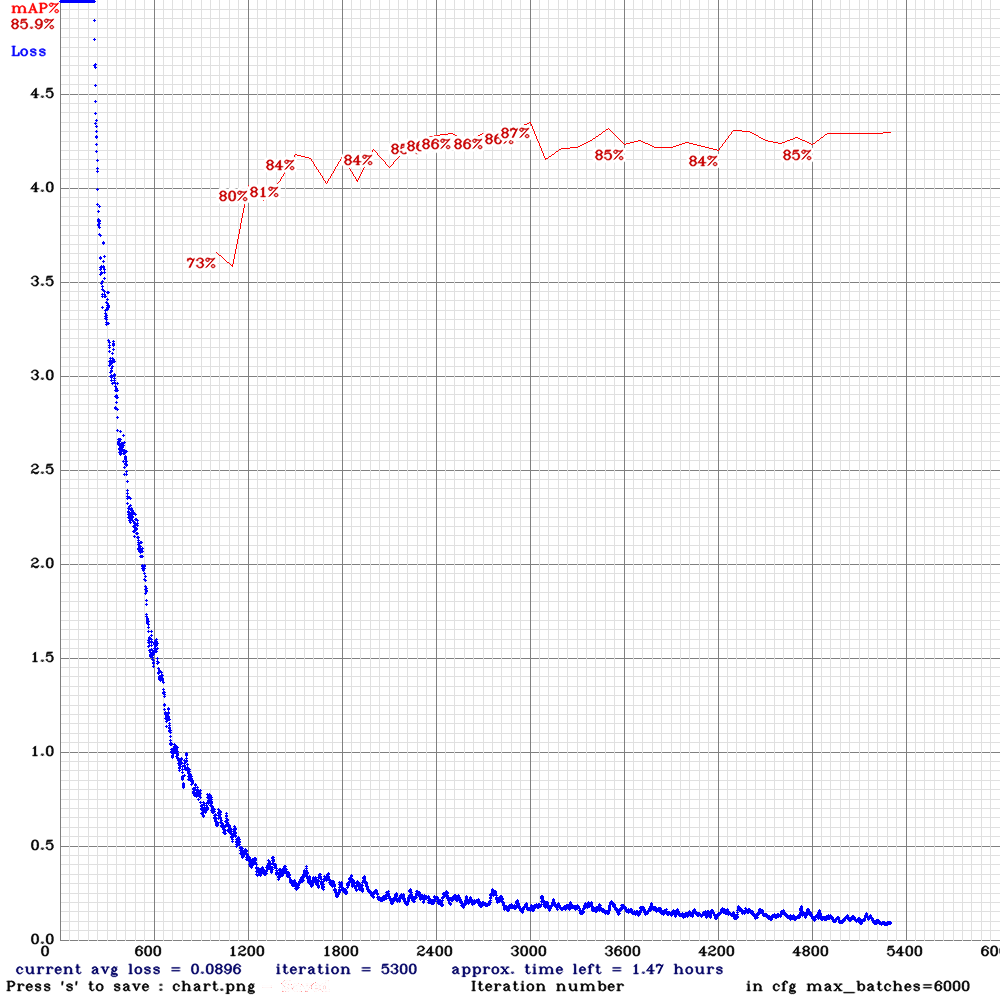
\includegraphics[width=0.4\textwidth]{pictures/painting_detection/training-v3.png}
    \caption{YOLOv3 trained on our custom dataset}
    \label{fig:training-v3}
\end{figure}

\begin{figure}[h!]
    \centering
        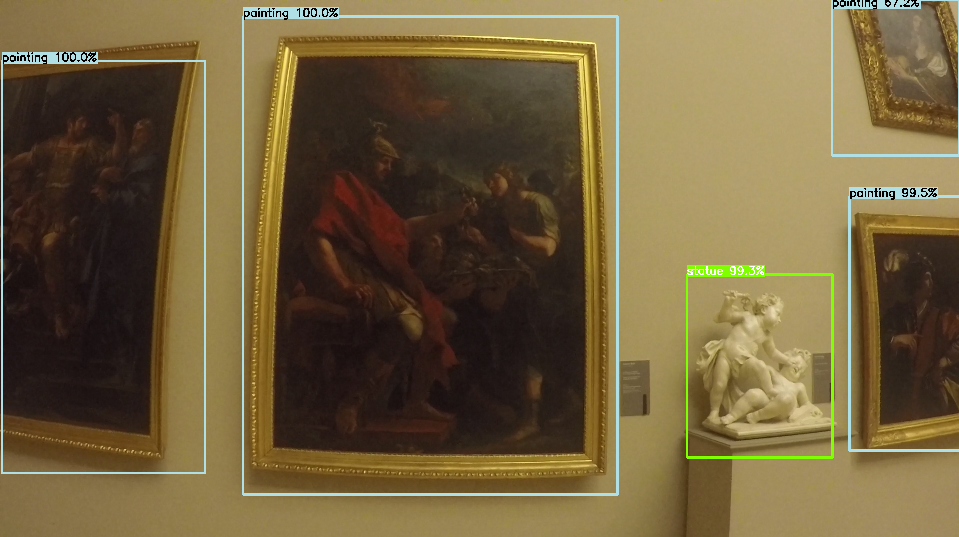
\includegraphics[width=0.5\textwidth]{pictures/painting_detection/yolo-detection2.PNG}
    \caption{Detection with YOLOv3}
    \label{fig:yolo_detection}
\end{figure}


\begin{figure*}[h]
    \minipage{0.32\textwidth}
      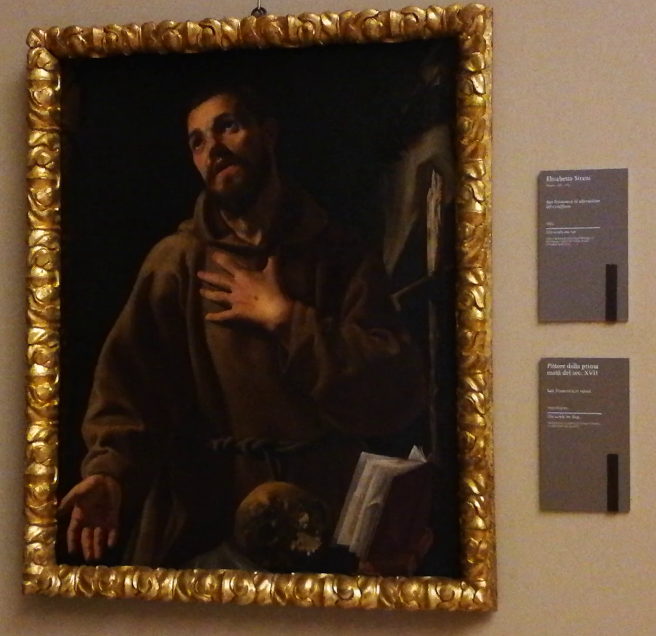
\includegraphics[width=\linewidth]{pictures/painting_detection/Frame.png}
      \caption*{Frame from video}\label{fig:Frame}
    \endminipage\hfill
    \minipage{0.32\textwidth}
      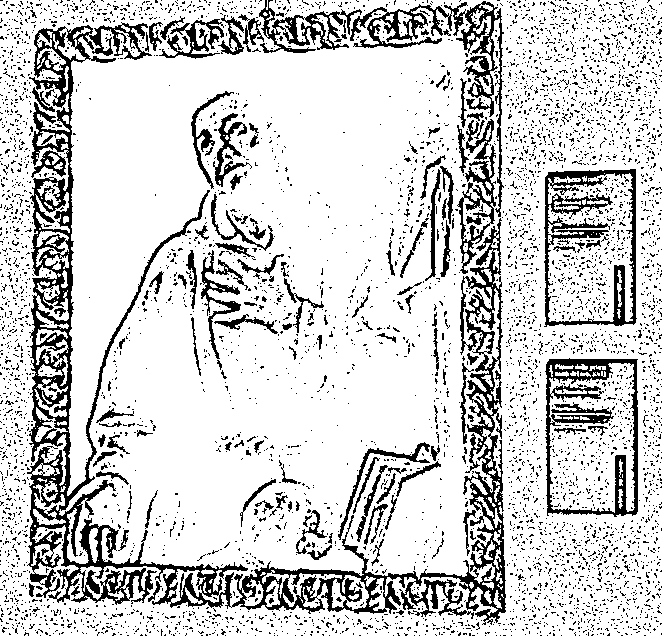
\includegraphics[width=\linewidth]{pictures/painting_detection/2-adaptive_threshold.PNG}
      \caption*{Adaptive threshold}\label{fig:adaptive_threshold}
    \endminipage\hfill
    \minipage{0.32\textwidth}%
      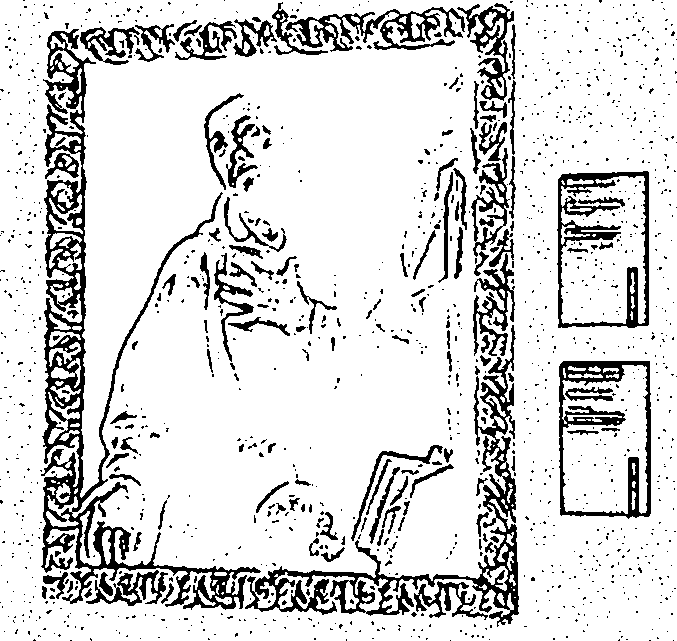
\includegraphics[width=\linewidth]{pictures/painting_detection/3-median_blur.PNG}
      \caption*{Median blur}\label{fig:median_blur}
    \endminipage
\end{figure*}


\begin{figure*}[h]

    \minipage{0.32\textwidth}
      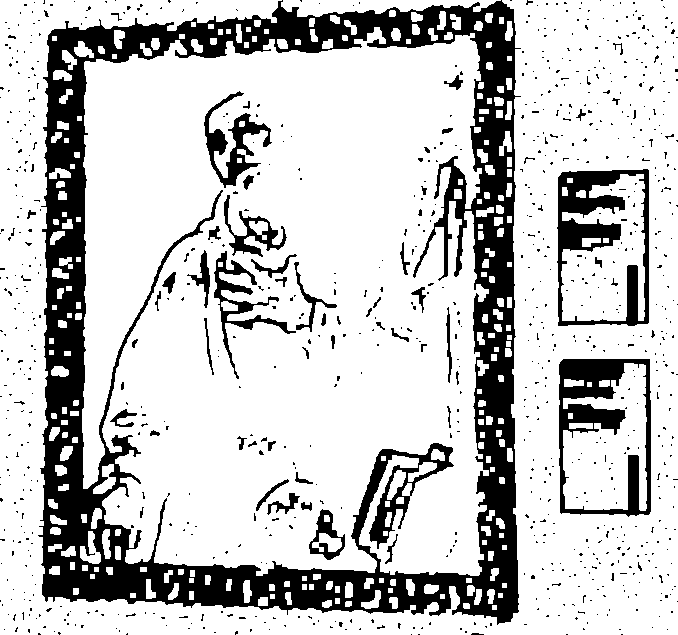
\includegraphics[width=\linewidth]{pictures/painting_detection/4-opening.PNG}
      \caption*{Opening}\label{fig:opening}
    \endminipage\hfill
    \minipage{0.32\textwidth}
    \vspace*{+4mm}
      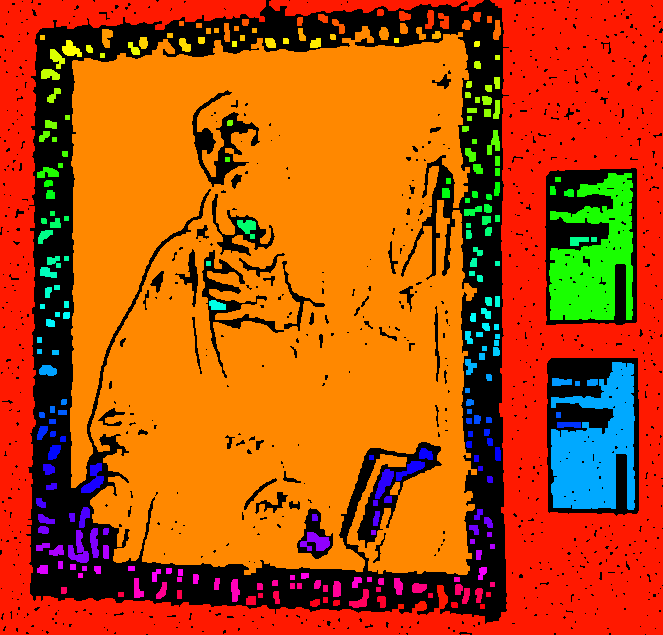
\includegraphics[width=\linewidth]{pictures/painting_detection/5-ccl.PNG}
      \caption*{Connected Component Labeling}\label{fig:ccl}
    \endminipage\hfill
    \minipage{0.32\textwidth}%
      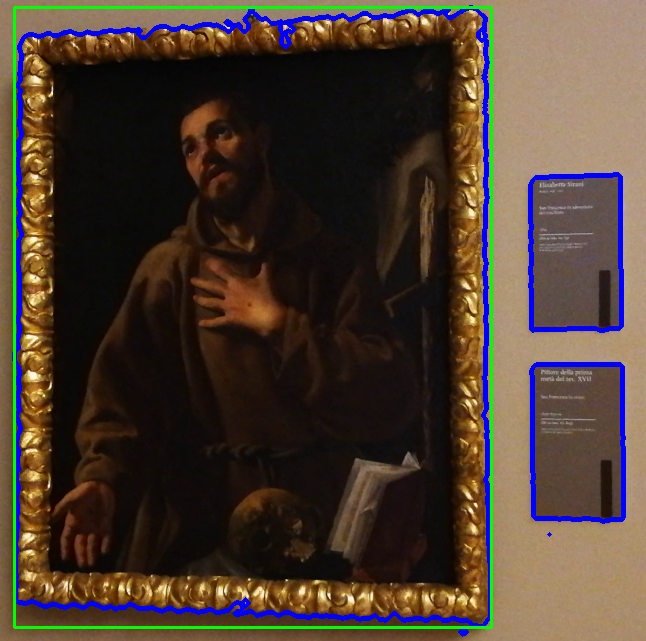
\includegraphics[width=\linewidth]{pictures/painting_detection/6-bbox.PNG}
      \caption*{Painting Detection}\label{fig:bbox}
    \endminipage
    \caption{Detection Pipeline without Neural Network} \label{fig:pipeline_detection}
\end{figure*}

\begin{figure*}[h]
    \minipage{0.45\textwidth}
      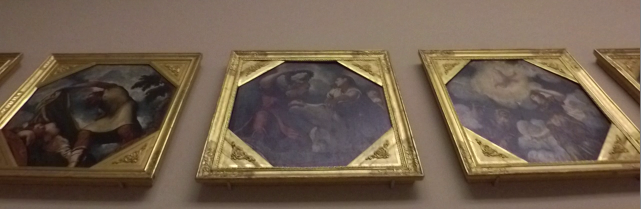
\includegraphics[width=\linewidth]{pictures/painting_detection/shadow1.PNG}
      \caption*{Image with shadow}\label{fig:shadow1}
    \endminipage\hfill
    \minipage{0.45\textwidth}
      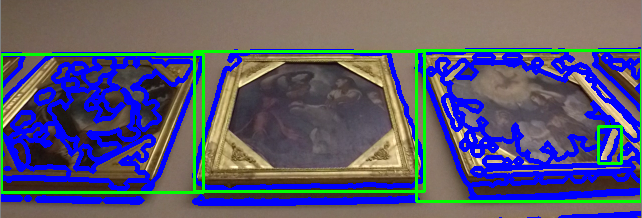
\includegraphics[width=\linewidth]{pictures/painting_detection/shadow2.PNG}
      \caption*{Not precise bounding box}\label{fig:shadow2}
    \endminipage\hfill
    \caption{Inaccurate detection due to the shadows}\label{fig:innaccurate_detection}
\end{figure*}







The detection of paintings, statues and person is done through a custom YOLOv3 neural network\cite{yolov3}.
Yolo is an architecture that provides a new approach to object detection, a single neural network predicts bounding boxes and class probabilities directly from full images in one evaluation.
In order to use this neural network we have labeled 1343 images, 805 of them have been used to train the network, 269 for the validation set and 269 for the test set, providing a total number of 3733 labels. The images of paintings and statues were taken by the frame extracted by some videos recorded in the Galleria Estense, for the person class was instead used a mix of labeled images taken from the previous videos and a some images of people in another museum.
The training has been performed with darknet \cite{darknet} taking the mAP every 1000 iterations \ref{fig:training-v3}, this allowed us to take the best weights that weren't affected by overfitting.
In the end we got a powerful neural network with high performance (Figure \ref{fig:yolo_detection}) and capable of a good generalization (see: Table \ref{tab:detection_performance}).
An important point is the data management: the train set, the validation set and the test set that have been used to achieve this performance were well balanced; 
if we hadn't used this approach the results would have been certainly worse and one or more classes wouldn't have been predicted in a correct way.



\begin{table*}[ht]
    \centering
\begin{tabular}{|c|c|c|c|c|}
\hline
\multicolumn{5}{|c|}{\textbf{Detection Performance}}       \\ \hline
\multicolumn{1}{|l|}{} & \textbf{Painting} & \textbf{Statue} & \textbf{Person} & \textbf{Overall} \\ \hline
\textbf{TP}        & 550     & 174     & 125     & 849     \\ \hline
\textbf{FP}        & 107     & 19      & 32      & 158     \\ \hline
\textbf{Precision} & 83,71\% & 90,16\% & 79,62\% & 84,31\% \\ \hline
\textbf{Recall}    & -       & -       & -       & 94\%    \\ \hline
\textbf{Average IoU}       & -       & -       & -       & 71\%    \\ \hline
\textbf{AP}        & 97,29\% & 98,61\% & 75,45\% & -       \\ \hline
\textbf{mAP}       & -       & -       & -       & 90,45\% \\ \hline
\end{tabular}
\caption{Detection Performance with YOLOv3} 
    \label{tab:detection_performance}
\end{table*}



\subsubsection{Comparison with previous technique}
In a previous pipeline (see Figure \ref{fig:pipeline_detection}) the detection was made without neural networks: the image was at first time transformed in a grey level image then was preprocessed and the contours were computed. After the creation of the gray level image was applied an adaptive threshold in order to take the significant edge, then was used a median blur for removing the noise which affected the image and the last processing was made by the erosion and the dilation.
The erosion and the dilation were combined together in order to create the opening, it was useful because with this technique the useless parts of the image were removed and the useful parts were increased.
When the preprocessing was terminated the pipeline had used the result to compute the foreground and the background with the Connected Component Labeling (see: \cite{Grana_ccl}).
After the image has been split in foreground and background the objects that had passed certain requirements and had achieved an entropy grater that a threshold was labeled as a painting, statue or person and the bounding box was drawn.
Despite this method worked well in the main scenery, it wasn't able to adapt to strong luminance variation, to manage the presence of shadows (Figure \ref{fig:innaccurate_detection}) and to generalize with all the classes. Many times the shadow was recognized as an object or as part of the painting and for this reason the IoU was computed with not optimal performance, this reason led us to choose to implement a neural network.

